
Les caractéristiques mécaniques du châssis connus, il est à présent possible de modéliser le système en utilisant les équations vues dans le chapitre \ref{chap:principe_physique}.
La totalité des fichiers Matlab se trouvent également en annexe \ref{annexe:git} ainsi que sur le git \ref{annexe:git}.

\section{Méthode et outils}
Les outils principaux utilisés dans le but de créer, de simuler ce système sont: Matlab, Simulink.
\section{Système à régler}

Cette section a pour objectif de définir le système à régler ainsi que les éléments influençant son comportement dynamique.
Comme présenté au chapitre \ref{chap:principe_physique}, les équations \ref{eq:ddtheta} et \ref{eq:ddx} décrivent le comportement physique du système.

Il existe cependant des différence avec la réalité qu'il est important d'expliquer.

\subsection{Moteur pas à pas}

Les équations de mouvement régissant le système utilisent comme paramètre d'entrée le couple moteur. Or, le système réel étant équipé de moteurs pas à pas, le couple produit n'est pas naturellement continu. Toutefois, l'utilisation d'un réglage en micro-pas fin ainsi que d'un lissage (voir \ref{subsection:drivers_moteurs}) permet d'obtenir un comportement proche d'un actionneur continu. Le moteur est donc modélisé par un couple continu afin de simplifier l'étude et la synthèse du régulateur.
\subsection{Modélisation de l'\acrshort{imu}}


Afin de reproduire fidèlement le comportement du robot réel, le modèle intègre une représentation simplifiée de l'\acrshort{imu}. Celle-ci ne se limite pas à la mesure de l'angle d'inclinaison, mais prend également en compte les caractéristiques physiques du capteur ainsi que son traitement numérique interne.

La modélisation repose sur trois éléments principaux :
\begin{itemize}
\item la position de l'\acrshort{imu} par rapport à l'axe de rotation des roues ;
\item la modélisation des mesures de l'accéléromètre et du gyroscope ;
\item le filtrage numérique permettant l'estimation de l'angle.
\end{itemize}

\subsubsection{Position de l'\acrshort{imu}}
\label{subsubsection:position_imu}
L'analyse du modèle CAO réalisée sous Fusion 360 a permis de déterminer avec précision la position de l'\acrshort{imu} par rapport à l'axe de rotation des roues (\ref{chap:mecanique}). Cette position est exprimée en coordonnées polaires par une distance $\rho$ et un angle $\phi$.

Le déport du capteur par rapport à l'axe de rotation induit des accélérations supplémentaires lors des mouvements du robot. En plus de l'accélération de translation du châssis, l'accéléromètre est soumis à une accélération tangentielle, proportionnelle à l'accélération angulaire $\ddot{\theta}$, ainsi qu'à une accélération centripète, proportionnelle au carré de la vitesse angulaire $\dot{\theta}$.

Les accélérations mesurées par l'accéléromètre sont ainsi obtenues en combinant :
\begin{itemize}
\item la projection de la gravité selon l'orientation du robot ;
\item l'accélération de translation du robot ;
\item les accélérations tangentielle et centripète dues au déport de l'\acrshort{imu}.
\end{itemize}

L'angle estimé à partir de l'accéléromètre est ensuite calculé à l'aide de la fonction $\mathrm{atan2}$.

\subsubsection{Modélisation du gyroscope}

Le gyroscope mesure directement la vitesse angulaire du robot autour de l'axe d'équilibrage. Dans le modèle, la mesure est supposée idéale et correspond directement à la vitesse angulaire issue du modèle dynamique :

$$
\omega = \dot{\theta}
$$

Les effets tels que le bruit de mesure ou la dérive du gyroscope ne sont pas pris en compte.

\subsubsection{Filtre complémentaire}

L'angle utilisé par le régulateur n'est pas directement issu de l'accéléromètre ou du gyroscope. Comme sur le robot réel, ces deux mesures sont fusionnées à l'aide d'un filtre complémentaire exécuté à une fréquence de 500~Hz, soit une période d'échantillonnage de $T_s = 2~\mathrm{ms}$.

À chaque période d'échantillonnage, la vitesse angulaire mesurée par le gyroscope est intégrée afin de prédire la nouvelle orientation du robot. Cette estimation est ensuite corrigée à l'aide de l'angle obtenu par l'accéléromètre selon la relation :
$$
\theta_{\mathrm{mes}}(k)
=
\alpha
\left(
\theta_{\mathrm{mes}}(k-1)
+
\omega(k)T_s
\right)
+
(1-\alpha)\theta_{\mathrm{acc}}(k)
$$

où $\alpha = 0.9$.

Ce filtre permet de combiner les avantages des deux capteurs : le gyroscope fournit une bonne estimation des variations rapides de l'orientation, tandis que l'accéléromètre permet de corriger la dérive du gyroscope à basse fréquence grâce à la mesure de la direction de la gravité.

\subsubsection{Intégration Matlab}

Le modèle de l'\acrshort{imu} ainsi que le filtre complémentaire sont ensuite implémentés dans Matlab/Simulink afin d'intégrer cette chaîne de mesure dans la simulation complète du robot.
\begin{figure}[H]
    \centering
    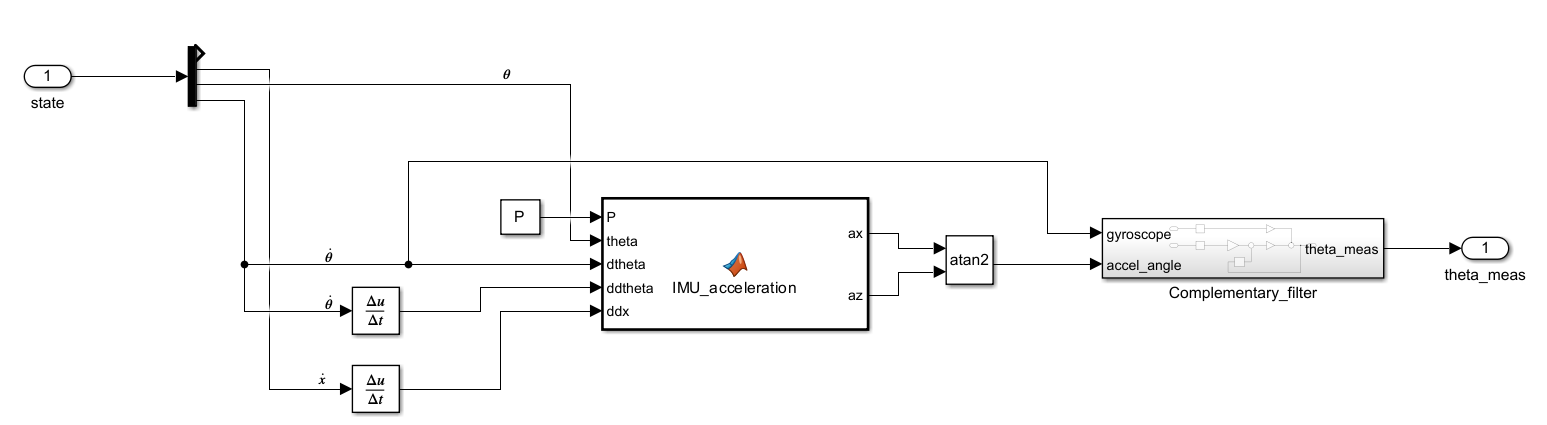
\includegraphics[width=1\textwidth]{assets/figures/simulink_schematic/IMU.png}
    \caption{Modèle de l'\acrshort{imu} dans Simulink}
    \label{fig:imu_simulink}
\end{figure}


\begin{figure}[H]
    \centering
    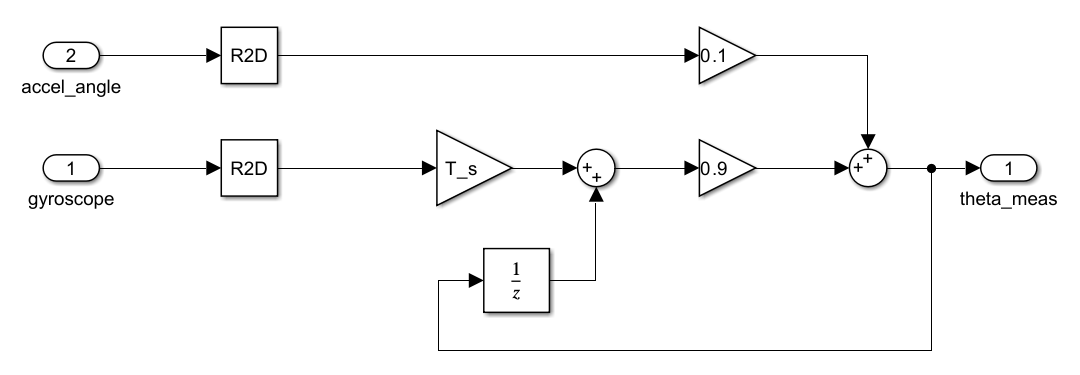
\includegraphics[width=1\textwidth]{assets/figures/simulink_schematic/complementary_filter.png}
    \caption{Implémentation du filtre complémentaire dans Simulink}
    \label{fig:complementary_filter}
\end{figure}


\section{Régulation}
\subsection{Structure de régulation retenue}

Dans une architecture classique de commande mécanique, la grandeur de commande appliquée aux actionneurs est généralement le couple moteur. Le régulateur calcule alors directement le couple nécessaire afin de modifier la dynamique du système. Cependant, cette approche n'est pas directement applicable au système étudié.

Le robot utilise des moteurs pas à pas dont la commande ne repose pas sur une régulation de couple. Les moteurs sont pilotés par des consignes de déplacement générées sous forme d'impulsions, la fréquence des impulsions définissant la vitesse de rotation et leur variation définissant l'accélération imposée aux roues.

La stratégie de régulation retenue est une structure en cascade composée de deux boucles :

\begin{itemize}
    \item une boucle externe de régulation de vitesse, dont l'objectif est de contrôler la vitesse linéaire du châssis ;
    \item une boucle interne de régulation d'angle, dont l'objectif est de maintenir l'inclinaison du robot à la valeur demandée.
\end{itemize}

La boucle externe compare la vitesse linéaire mesurée du robot avec la consigne de vitesse :

$$
e_v = v_{\mathrm{ref}} - v
$$

Cette erreur est appliquée à un régulateur permettant de déterminer l'angle d'inclinaison souhaité :

$$
\theta_{\mathrm{ref}} = C_v(e_v)
$$

L'inclinaison demandée représente alors une consigne d'accélération indirecte. En effet, pour accélérer dans une direction donnée, le robot doit volontairement s'incliner afin de créer une composante du poids permettant de générer le mouvement.

La boucle interne compare ensuite l'angle désiré avec l'angle mesuré par l'\acrshort{imu} :

$$
e_{\theta} = \theta_{\mathrm{ref}}-\theta
$$

Le régulateur d'angle calcule l'accélération nécessaire des roues :

$$
a_{\mathrm{roues}} = C_{\theta}(e_{\theta})
$$

Cette accélération est ensuite intégrée et transmise sous forme de vitesse aux drivers moteurs.

La structure complète de commande est donc :

$$
v_{\mathrm{ref}}
\rightarrow
(v_{\mathrm{ref}}-v)
\rightarrow
\theta_{\mathrm{ref}}
\rightarrow
(\theta_{\mathrm{ref}}-\theta)
\rightarrow
a_{\mathrm{roues}}
\rightarrow
\text{moteurs pas à pas}
$$

Cette architecture présente l'avantage de découpler la dynamique de déplacement et la dynamique d'équilibrage. La boucle interne, plus rapide, garantit la stabilité du robot tandis que la boucle externe impose le comportement global en vitesse.
\subsection{Calcul du couple moteur équivalent}

Le modèle dynamique obtenu précédemment permet d'établir la relation entre le couple moteur appliqué aux roues et l'accélération du châssis. Bien que la commande réelle du robot soit réalisée en accélération par l'intermédiaire des moteurs pas à pas, le calcul du couple équivalent permet de vérifier la cohérence physique de la commande.

L'équation dynamique selon l'axe horizontal est donnée par :

\[
\ddot{x} =
\frac{1}{d_1}
\left(
aI_O\dot{\theta}^2\sin(\theta)
-
a^2g\sin(\theta)\cos(\theta)
+
T
\left(
\frac{I_O}{r}+a\cos(\theta)
\right)
\right)
\]

avec :

\[
d_1=I_Om_O-a^2\cos^2(\theta)
\]

Le couple moteur peut être obtenu en isolant le terme associé à l'actionneur :

\[
T=
\frac{
d_1\ddot{x}
-
aI_O\dot{\theta}^2\sin(\theta)
+
a^2g\sin(\theta)\cos(\theta)
}
{
\frac{I_O}{r}+a\cos(\theta)
}
\]


\subsection{Intégration Matlab}

La figure \ref{fig:input_simulink} montre l'intégration des deux régulateurs imbriqués. Il s'agit ici de régulateurs analogique saturés. Les valeurs de saturations
restent à définir.
Ces derniers sont également paramétrés avec un anti-windup.
On y voit également l'intégration du signal d'entré principal, ici $v_{target}$ soit la consigne de vitesse.

A la sortie de cette image, un bloc ZOH, (Zero Order Hold), permet de cadancer le système à la fréquene souhaitée (permettant un représentation fidèle de la réalité.)
Le signe négatif appliqué à la sortie du régulateur d'angle permet d'adapter la commande à la dynamique du pendule inversé. En effet, une correction de l'inclinaison nécessite un déplacement des roues dans la direction opposée au mouvement angulaire souhaité. Cette inversion assure donc la cohérence entre la consigne d'accélération des roues et le sens de réaction mécanique du robot.
\begin{figure}[H]
    \centering
    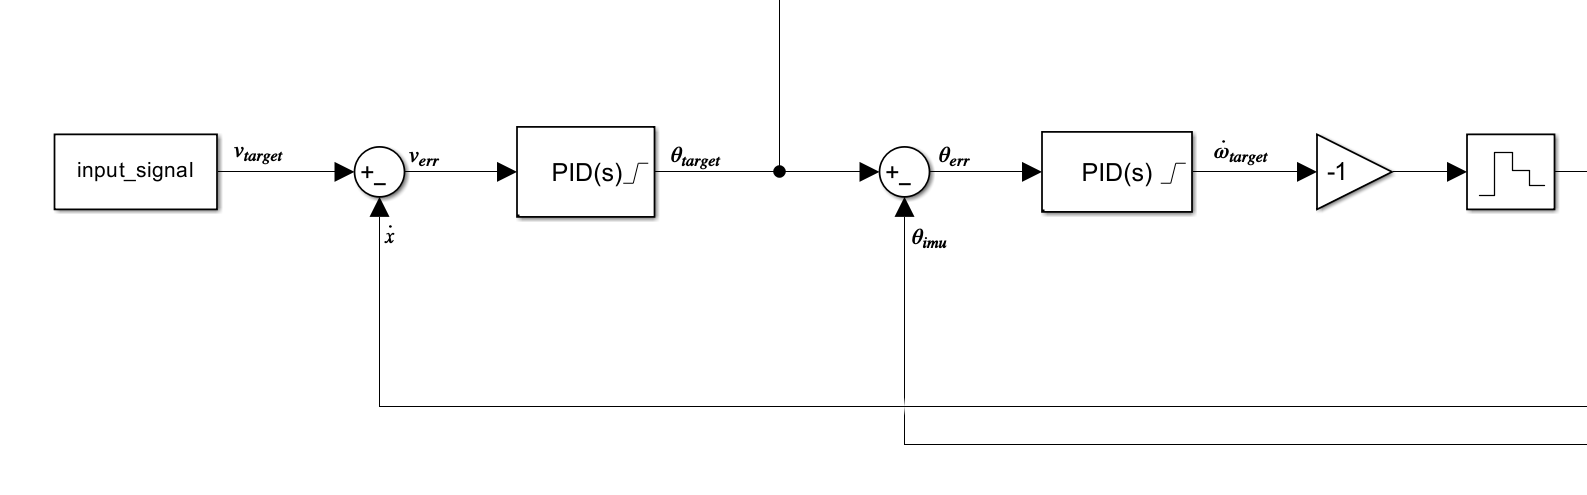
\includegraphics[width=1\textwidth]{assets/figures/simulink_schematic/input.png}
    \caption{Modèle régulateurs PID}
    \label{fig:input_simulink}
\end{figure}

La figure \ref{fig:linear_speed} présente la lecture de la vitesse linéaire. Cette dernière est entièrement déterminée par la consigne de vitesse appliquée aux moteurs pas à pas. 
Il s'agit également d'une adaptation permettant de modéliser plus fidèlement le comportement du système réel.

Les valeurs obtenues par l'intégration de la consigne d'accélération sont identiques à celles obtenues à partir du modèle physique \texttt{robot\_dynamics}.
\begin{figure}[H]
    \centering
    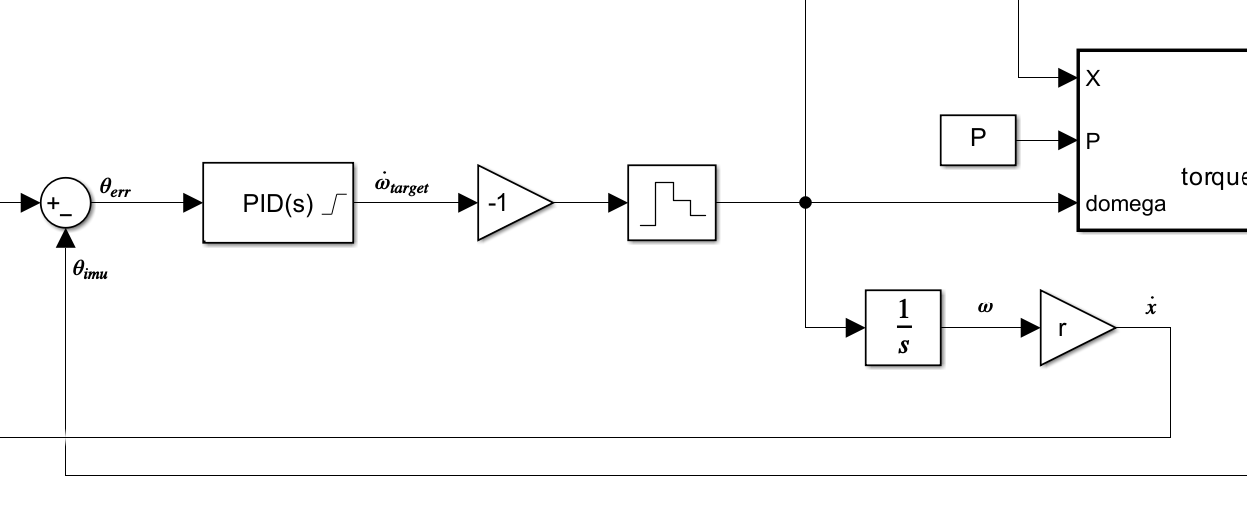
\includegraphics[width=1\textwidth]{assets/figures/simulink_schematic/omega_reading.png}
    \caption{Lecture de vitesse linéaire}
    \label{fig:linear_speed}
\end{figure}

La figure \ref{fig:torque_physics} présente l'intégration des deux principaux blocs de calcul. Le premier, \texttt{torque\_computation}, permet de déterminer le couple à partir de l'accélération, tandis que le second, \texttt{robot\_dynamics}, intègre les équations du modèle physique présentées dans la section \ref{chap:principe_physique}.

Cette figure illustre également l'implémentation du bloc \acrshort{imu}, placé en sortie du calcul dynamique afin de simuler les mesures fournies par le capteur inertiel.
\begin{figure}[H]
    \centering
    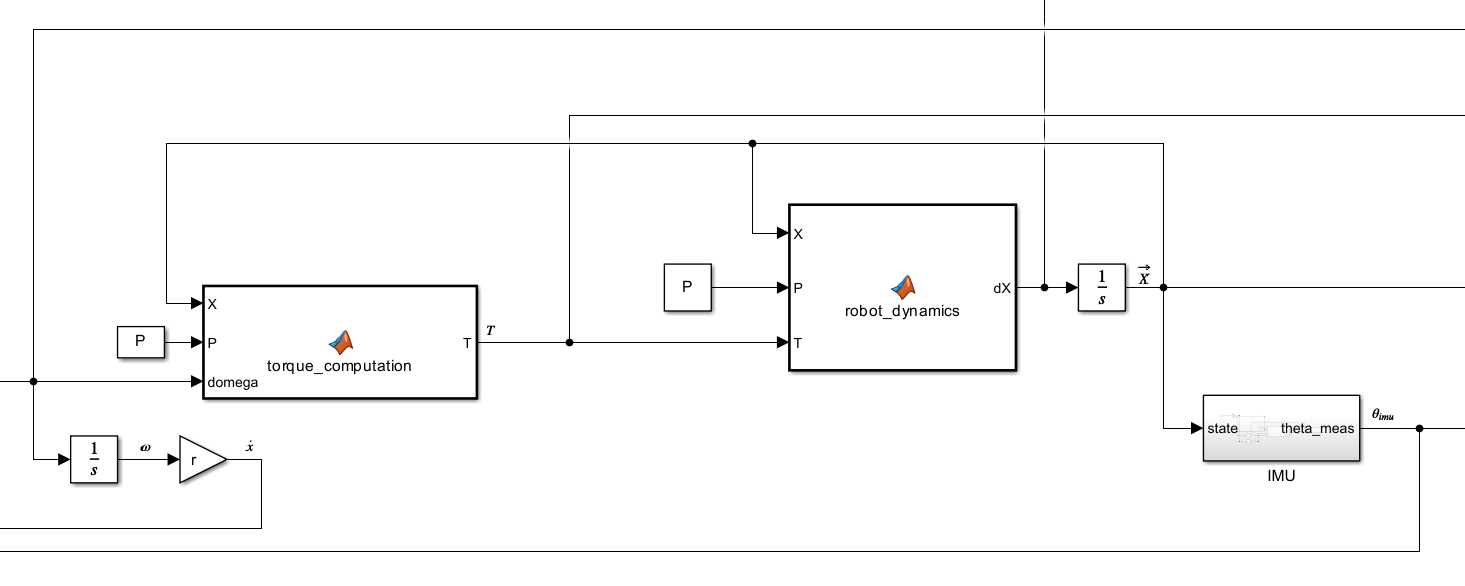
\includegraphics[width=1\textwidth]{assets/figures/simulink_schematic/torque_physics.png}
    \caption{Calcul du couple, modèle théorique}
    \label{fig:torque_physics}
\end{figure}

La constante \(P\) présente dans les figures ci-dessus représente un vecteur de paramètres. 
L'intégralité de ces paramètres se trouve dans le fichier \texttt{complete\_parameters.m}. 
Le vecteur \(\vec{X}\) correspond au vecteur d'état du système, défini par :

\[
\vec{X} =
\begin{bmatrix}
x \\
\dot{x} \\
\theta \\
\dot{\theta}
\end{bmatrix}
\]

où \(x\) représente la position linéaire, \(\dot{x}\) sa dérivée temporelle, \(\theta\) la position angulaire et \(\dot{\theta}\) la vitesse angulaire.